\section{Global Minimum Cut}
\label{sec:global}

Let~$G$ be undirected. We now turn our attention computing the global minimum cut of~$G$.
To work with topology in computing a minimum cut, we use the following lemma which is similar very similar to Lemma~\ref{lem:cut-duality}.
We say a null-homologous even subgraph~$\eta$ is a \EMPH{separating subgraph} if it contains at least one edge.

\begin{lemma}
\label{lem:mincut-z2}
Let~$G$ be an edge-weighted undirected graph embedded on a surface~$\Sigma$ without boundary, and let~$C$ be a minimum cut in~$G$.
Then~$C^*$ is a minimum weight separating subgraph of~$G^*$.
\end{lemma}

\begin{proof}
  Let~$C$ be an arbitrary cut in~$G$.  The cut partitions the vertices of $G$
  into two disjoint subsets~$S$ and~$T$. Therefore, the dual subgraph~$C^*$
  partitions the faces of~$G^*$ into two disjoint subsets~$S^*$ and~$T^*$.
  Further,~$C^*$ is the boundary of the union of faces in~$S^*$, implying
  that~$C^*$ is null-homologous in~$\Sigma$ and therefore separating.

  Conversely, let~$C^*$ be an arbitrary separating subgraph of~$G^*$.
  As~$C^*$ is null-homologous, it is the boundary of a subset of the faces
  of~$G^*$.  Moreover, because $C^*$ is non-empty, it must be the boundary of
  a \emph{proper, non-empty} subset of faces.  Let $s^*$ and $t^*$ be faces
  of $G^*$ on either side of $C^*$.  Any path from~$s$ to~$t$ in the primal
  graph~$G$ must traverse at least one edge of~$C$.  We conclude that~$C$ is
  a cut (in particular, an $s,t$-cut).
\end{proof}

Fix an undirected graph~$G=(V,E)$, a non-negative weight function ${w\colon E\to \Real}$, and a cellular embedding of~$G$ on a surface~$\Sigma$ of genus~$g$ with at least two faces.  In light of Lemma \ref{lem:mincut-z2}, we focus our attention on finding a minimum weight separating subgraph of~$G$. 

Our algorithm separately considers two cases, illustrated in Figure~\ref{fig:global_cases}. Exactly one of these cases must apply to the minimum weight separating subgraph.
\begin{enumerate}
  \item
    Some minimum weight separating subgraph consists of a single contractible simple cycle.
  \item
    Every minimum weight separating subgraph can be decomposed into non-contractible simple cycles.
\end{enumerate}
%
\begin{figure}[h]
\centering
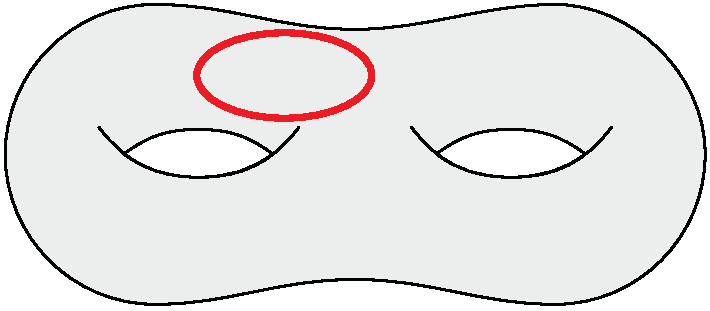
\includegraphics[height=1in]{Fig/shortcon2}\qquad
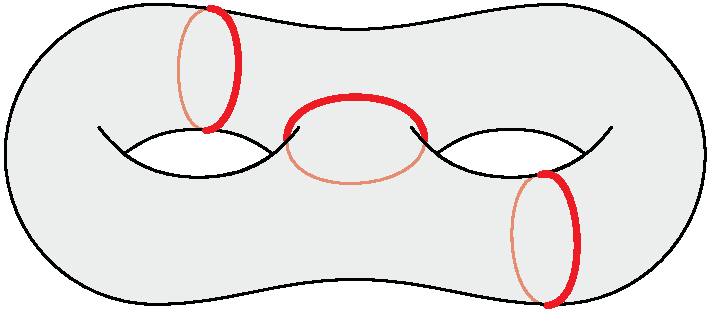
\includegraphics[height=1in]{Fig/homologous1}
\caption{Two types of minimum weight separating subgraphs: a contractible cycle and otherwise.}
\label{fig:global_cases}
\end{figure}
%

Throughout the rest of this section, we describe two subroutines to find minimum weight separating subgraphs that are designed with their corresponding condition in mind. If the corresponding condition does hold, the subroutine will return a separating subgraph with weight at most that of the minimum weight separating subgraph. Otherwise, the subroutine may return a higher weight separating subgraph. By running both subroutines and returning the best result, we find a minimum weight separating subgraph no matter which category it falls into.

%%%%%%%%%%%%%%%%%%%%%%%%%

\subsection{Contractible cycle}
\label{sec:global_contractible}

We begin by describing an algorithm to handle the case where some minimum weight separating subgraph is a contractible simple cycle.
We begin by borrowing a result of Cabello~\cite[Lemma 4.1]{c-fscss-10}.

\begin{lemma}[Cabello~\cite{c-fscss-10}]
\label{lem:disjoint-tight-arc}
Let $\alpha$ be a tight arc or tight cycle on $G$.  There exists a shortest contractible simple cycle that does not cross $\alpha$.
\end{lemma}

\begin{corollary}
\label{cor:disjoint-sep-cycle}
The shortest contractible simple cycle and the shortest non-separating cycle in $G$ do not cross.
\end{corollary}

\begin{figure}[h]
\centering
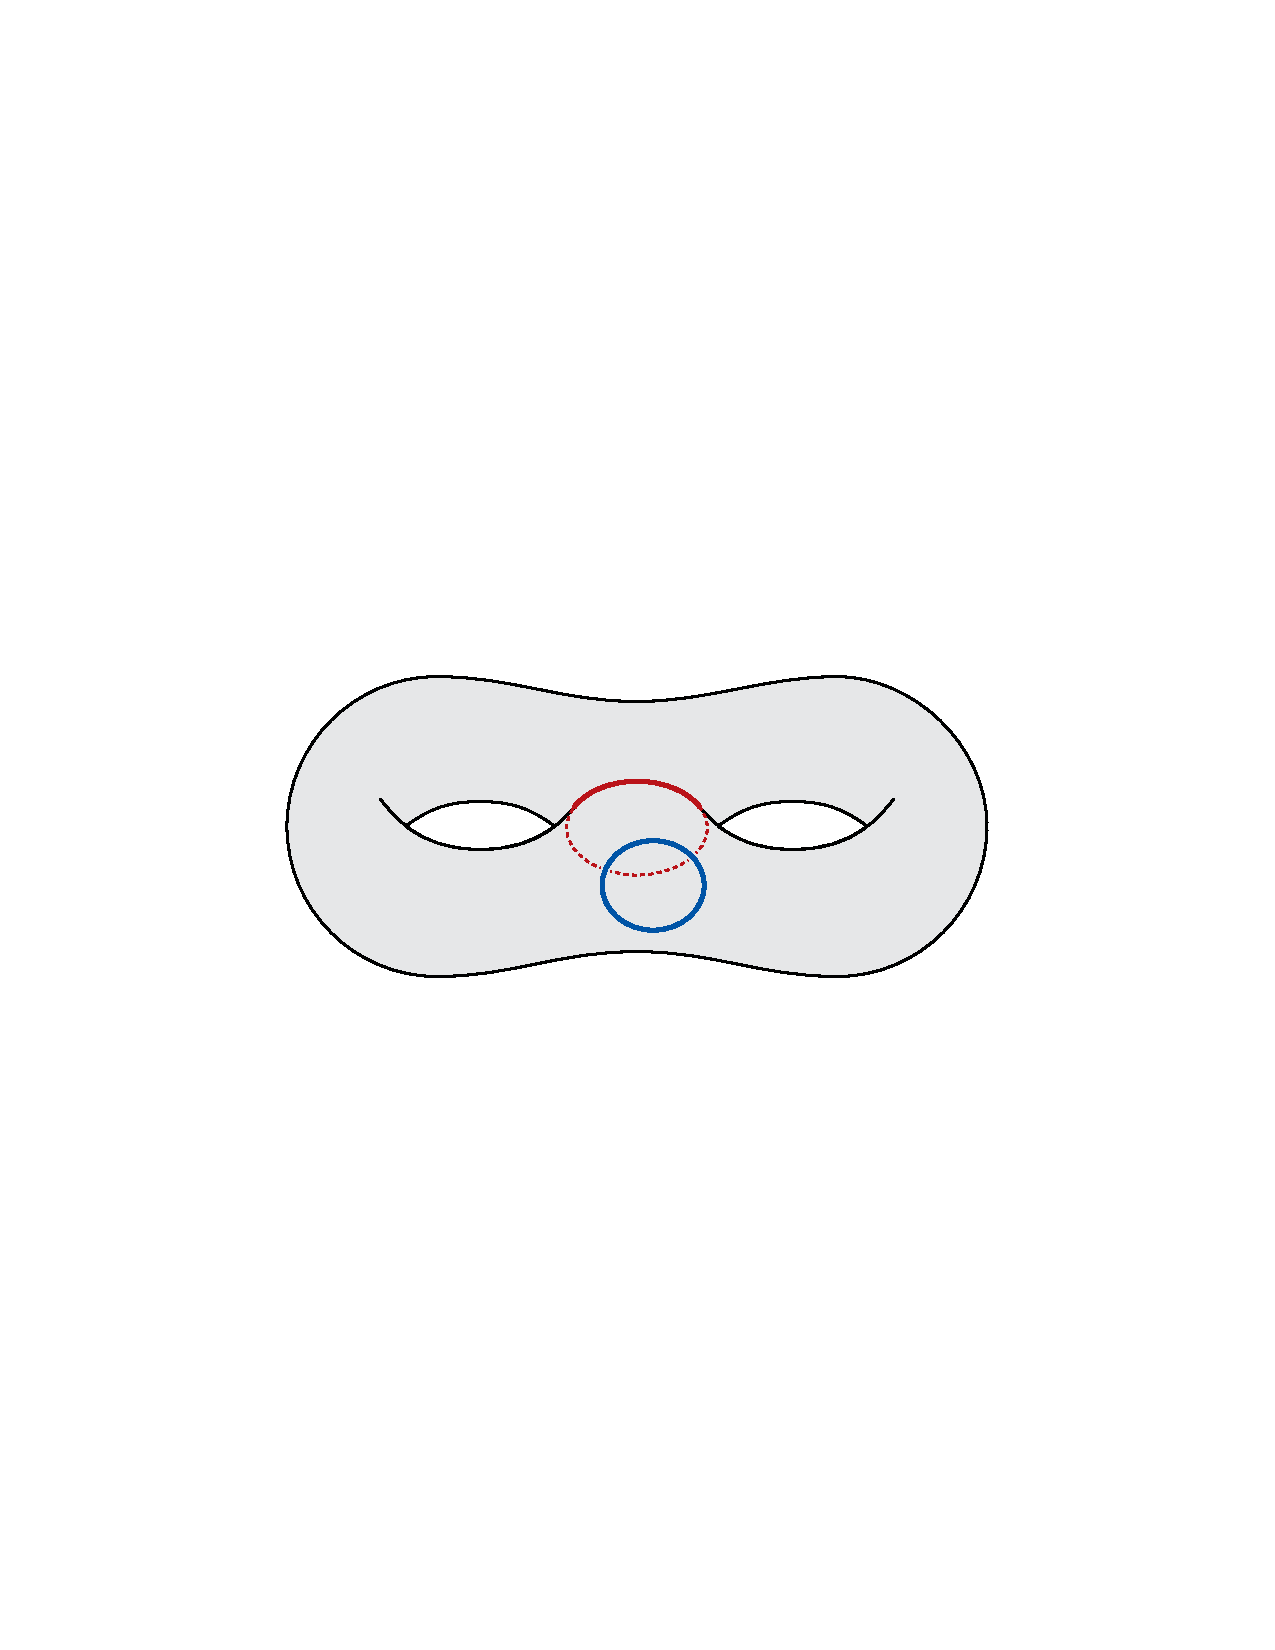
\includegraphics[height=1.2in]{Fig/shortcon-vs-shortnonsep}
\caption{A shortest contractible simple cycle does not cross some shortest non-separating cycle.}
\label{fig:global_shortcon-vs-shortnonsep}
\end{figure}

Cabello~\cite{c-fscss-10} uses these observations in order to compute a shortest contractible simple cycle in a surface embedded graph.
Unfortunately his algorithm takes~$\Omega(n^2)$ time, because his algorithm must return a shortest contractible simple cycle even if it is not a minimum weight separating subgraph.
Cabello \etal~\cite{cdem-fotc-10} use a similar procedure to find a shortest \emph{enclosing cycle} which bounds a non-empty set of faces.
While this procedure can be modified to run in~$g^{O(g)} n \log \log n$ time, it may return a cycle that is actually trivial after taking the symmetric difference over all its edges with multiplicity.
The cycle returned may not be a separating subgraph as per our definition.

Our algorithm will make use of the cutting operation ($\snip$) along tight cycles and arcs in~$G$.
\note{TODO: Define $\snip$ in the prelims.}
The following lemma implies it is safe for our algorithm to find minimum weight separating subgraphs in snipped copies of~$\Sigma$.
\begin{lemma}
\label{lem:global_null-homologous-projections}
Let~$\alpha$ be an arbitrary simple cycle or arc in~$G$. Let
${\Sigmasnip = \Sigma \snip \alpha}$ and let~$\Gsnip = G \snip \alpha$. Any null-homologous even subgraph~$\gammasnip$ in~$\Gsnip$ projects to a null-homologous even subgraph in~$G$.
\end{lemma}
\begin{proof}
Let~$\gammasnip$ be an arbitrary null-homologous even subgraph in~$\Gsnip$ and let~$\gamma$ be its projection in~$G$.
Subgraph~$\gamma$ bounds a subset of faces~$F_{\subsnip}$ in~$\Gsnip$. 
Let~$F$ be the projection of~$F_{\subsnip}$ into~$G$.
We will argue that~$\gamma$ bounds~$F$, proving the lemma.

Consider any edge~$e = f | g$ on the boundary of~$F$. If~$f$ and~$g$ still lie adjacent along~$e$ in~$\Gsnip$, then~$e$ bounds~$F_{\subsnip}$ and appears in~$\gamma$. If~$e$ separates a face~$f$ from the boundary of~$\Gsnip$, then~$e$ still appears in~$\gamma$.

Now consider any edge~$e$ in~$\gammasnip$. Suppose~$e$ does not lie along~$\alpha$ so that its projection appears in~$\gamma$. Edge~$e$ separates two faces~$f$ and~$g$ in~$\Gsnip$, and exactly one of those faces appears in~$F$. Now suppose~$e$ does lie along~$\alpha$. Edge~$e$ separates face~$f \in F$ from the boundary of~$\Gsnip$. The projection of~$e$ may separate~$f$ from another face~$g$. If~$g$ exists and is also in~$F$, then there exists another edge~$e'$ in~$\Gsnip$ that separates~$g$ from the boundary of~$\Gsnip$. The projections of~$e$ and~$e'$ cancel each other when taking the symmetric difference so their projection does not appear in~$\gamma$. Finally, if~$g$ does not exist or~$g$ is not a member of~$F$, then there is not another edge that shares a projection with~$e$. The projection of~$e$ will exist in~$\gamma$.
\end{proof}

We now present the main result of this section.
\begin{lemma}
\label{lem:contractible-alg}
There exists a~$g^{O(g)} n \log \log n$ time algorithm that computes a minimum weight separating subgraph if any such subgraph is a contractible simple cycle. If not, the algorithm either returns some separating subgraph (that may not be minimum weight) or nothing.
\end{lemma}

\begin{proof}
Our algorithm begins by computing a shortest non-separating cycle~$\alpha$ in $G$ in $g^{O(g)}n \log \log n$ time, using a modification of an algorithm of Kutz~\cite{k-csnco-06} by Italiano \etal~\cite{insw-iamcmf-11} or using a recent $2^{O(g)}n \log \log n$ time algorithm of Fox~\cite{f-sntcd-13}.  The surface $\Sigma \snip \alpha$ has two boundary cycles $\alpha'$ and $\alpha''$.

It then computes a system $P$ of tight arcs anchored on $\alpha'$ and $\alpha''$ in $O(n)$ time as described in Section~\ref{sec:characterizing_crossings}.
\note{Again, verify that the set of arcs can be computed in linear time this way.}
Let $\Gsnip$ denote the planar graph $G \snip (\alpha \cup P)$; this graph has $O(gn)$ vertices.

Pick an arbitrary edge $e$ of $\alpha$, and let $e_1$ and $e_2$ be distinct copies of $e$ in~$\Gsnip$.  Let $\gamma_1$ and $\gamma_2$ be the shortest simple cycles in the  subgraphs $\Gsnip \backslash e_1$ and $\Gsnip \backslash e_2$, respectively.  Our algorithm computes both~$\gamma_1$ and~$\gamma_2$ in $O(gn \log\log n)$ time using the algorithm of \L\c{a}cki and Sankowski~\cite{ls-mcsc-11}. Note that graphs~$\Gsnip \backslash e_1$ and~$\Gsnip \backslash e_2$ may not contain any cycles. In this case,~$\Gsnip$ contains no simple cycles. Corollary~\ref{cor:disjoint-sep-cycle} and Lemma~\ref{lem:disjoint-tight-arc} imply~$G$ does not contains any contractible simple cycles to begin with and our algorithm returns nothing. For the rest of this section, we assume~$\gamma_1$ and~$\gamma_2$ are well defined.

\begin{figure}[h]
\centering
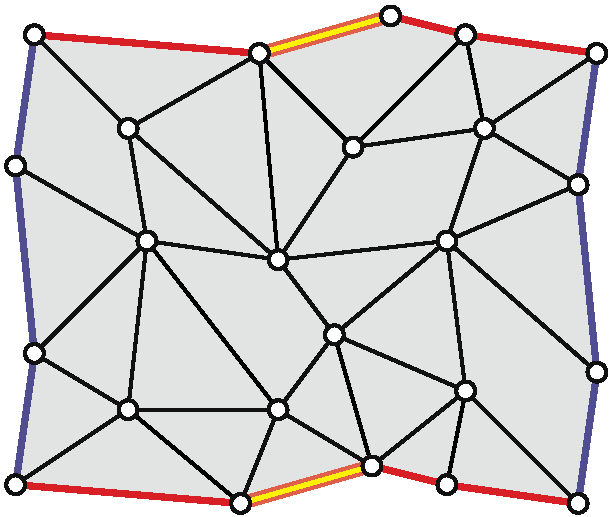
\includegraphics[height=1.2in]{Fig/forbidden-pair}
\caption{At least one copy of $e$ is forbidden in the planarized graph.}
\label{fig:global_forbidden-pair}
\end{figure}

Let~$\gamma$ be the shorter of the cycles~$\gamma_1$ and $\gamma_2$.  By multiple instantiations of Lemma~\ref{lem:global_null-homologous-projections}, cycle~$\gamma$ projects to a null-homologous closed walk $\gamma'$ in the original graph $G$, which may or may not be simple.
Our algorithm returns the symmetric difference over all edges in~$\gamma'$. The outer face of $\Gsnip$ is the only face that is not also a face of~$G$.
It follows that the only separating cycle in $\Gsnip$ that is not a separating subgraph in $G$ is the boundary of outer face.  Because $\gamma$ avoids at least one edge of the outer face, the carrier of $\gamma'$ must be non-empty. If our algorithm returns anything, it must return a separating subgraph.

Now, suppose some minimum weight separating subgraph of~$G$ is a contractible simple cycle. Corollary~\ref{cor:disjoint-sep-cycle} and Lemma~\ref{lem:disjoint-tight-arc} imply that some shortest contractible simple cycle $\sigma$ in $G$ crosses neither~$P$ nor $\alpha$.  (We emphasize that our algorithm does not necessarily compute~$\sigma$.)  This cycle $\sigma$ appears as a simple cycle in $\Gsnip$ that avoids at least one of the edges $e_1$ or $e_2$.  Thus, $\sigma$ cannot be shorter than $\gamma$, and our algorithm returns a minimum weight separating subgraph.
\end{proof}

%%%%%%%%%%%%%%%%%%%%%%%%%%%%%%%%%%%%

\subsection{Non-contractible components}
\label{sec:global_non-contractible}
Next, we consider the case where all minimum weight separating subgraphs contain components that are non-contractible. The following lemma is the key result of this section and could likely have applications beyond this work.
\begin{lemma}
\label{lem:global_split-nocross}
Let~$\sigma$ be a minimum weight separating subgraph, and let~$f$ be any face of~$G$.
Let~$\gamma$ be a closed walk on~$G$ that lies in the closure of the opposite component of~$f$ in~$\Sigma \setminus \sigma$, and let~$\eta$
be a shortest even subgraph homologous to~$\gamma$.
There exists a minimum weight separating subgraph~$\sigma'$ (possibly~$\sigma$) such
that~$\eta$ lies in the closure of the opposite component of~$f$ in~$\Sigma \setminus \sigma'$. (See Figure~\ref{fig:global_nonsep-vs-shortsep}.)
\end{lemma}
\begin{figure}[h]
\centering
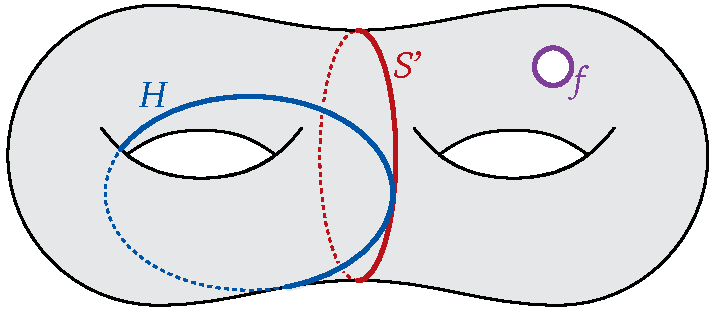
\includegraphics[height=1.2in]{Fig/nonsep-vs-shortsep}
\caption{The setting of Lemma~\ref{lem:global_split-nocross}. A~$\Z_2$-minimal even subgraph~$\eta$ is separated from face~$f$ by a minimum weight separating subgraph~$\sigma'$.}
\label{fig:global_nonsep-vs-shortsep}
\end{figure}
\begin{proof}
If~$\sigma$ fits the requirement that~$\eta$ lies in the closure of the opposite component of~$f$ in~$\Sigma \setminus \sigma$, then we are done. Assume otherwise.
The subgraph~$\sigma$ separates the faces of~$G$ into two non-empty sets.  Call the faces in the component of~$\Sigma \setminus \sigma$ containing~$f$ the \emph{far} faces and call the rest of the faces  \emph{near}.  Similarly, the even subgraph $\eta \oplus \gamma$ is null-homologous and separates the faces of $G$ into two subsets; call the faces in the subset containing~$f$ \emph{black} and the others \emph{white}.

Let~$\sigma'$ be the boundary of the union of the far black faces in $G$.
By definition,~$\sigma'$ is a null-homologous even subgraph.  By assumption, $\eta$ has edges that are incident to two far faces, but $\gamma$ does not; thus, there is at least one far black face~$f$.  Since there is also at least one near face, $\sigma'$ is non-empty. 
No edge of~$\eta$ lies between two far black faces so~$\eta$ lies in the closure of the opposite component of~$f$ in~$\Sigma \setminus \sigma'$. We claim~$\sigma'$ is a minimum weight even subgraph.

For the sake of contradiction, suppose~$\sigma'$ is not a minimum weight even subgraph.
Because both~$\sigma'$ and $\sigma$ are null-homologous, the even subgraph $\eta' = \eta \oplus \sigma' \oplus \sigma$ is homologous to $\eta$, and therefore to $\gamma$.

For any subgraph~$H$ of $G$, let $w(H)$ denote the sum of the weights of the edges of $H$.  We now prove that $w(\sigma') + w(\eta') \leq w(\eta) + w(\sigma)$ by bounding the contribution of each edge $e \in E(G)$ to both sides of the inequality.  Note that both $\sigma'$ and $\eta'$ are subgraphs of $\sigma\cup \eta$; moreover, $\sigma' \oplus \eta' = \sigma \oplus \eta$.  There are three cases to consider.
\begin{itemize}
\item
If $e \not\in \eta \cup \sigma$, then $e$ contributes $0$ to both sides of the inequality.
\item
If $e \in \sigma \oplus \eta$, then $e \in \sigma' \oplus \eta'$.  In this case, $e$ contributes $w(e)$ to both sides of the inequality.
\item
If $e \in \sigma \cap \eta$, then $e$ contributes exactly $2w(e)$ to the right side of the inequality.  Trivially, $e$ contributes at most $2w(e)$ to the left side.
\end{itemize}

On the other hand, because $\sigma'$ is not a minimum weight separating subgraph, we must have $w(\sigma') > w(\sigma)$. 
It immediately follows that $w(\eta') < w(\eta)$, which contradicts the minimality of $\eta$.
\end{proof}

We now present the main result of this section, concluding the description of our algorithm for computing minimum weight separating subgraphs and minimum cuts.
\begin{lemma}
  \label{lem:global_split-alg}
  There exists a~$g^{O(g)} n \log \log n$ time algorithm that computes a minimum weight separating subgraph if every minimum weight separating subgraph can be decomposed into non-contractible simple cycles. If not, the algorithm either returns some separating subgraph (that may not be minimum weight) or nothing.
\end{lemma}
\begin{proof}
Our algorithm begins by picking an arbitrary face~$f$ of~$G$. Let~$\sigma$ be an arbitrary minimum weight separating subgraph.
We argue that there exists a non-separating closed walk~$\gamma$ in~$G$ that lies in the closure of the opposite component of~$f$ in~$\Sigma \setminus \sigma$.

By assumption,~$\sigma$ can be decomposed into simple cycles, each of which is non-contractible. Suppose~$\sigma$ consists of more than one cycle. None of the cycles are null-homologous, because we could remove a single null-homologous cycle from~$\sigma$ to lower its cost without changing it homology class.
In this case,~$\gamma$ is simply one of the cycles in~$\sigma$'s decomposition. Now, assume~$\sigma$ consists of a single simple cycle. Cycle~$\sigma$ is not contractible by assumption, so neither component of $\Sigma \setminus \sigma$ is planar. The closure of the component opposite~$f$ has non-zero genus and therefore contains a non-separating closed walk in~$\Sigma$.

Let~$\eta$ be a shortest even subgraph homologous to~$\gamma$.
By Lemma~\ref{lem:global_split-nocross}, we may assume without loss of generality that~$\eta$ lies in the closure of the opposite component of~$f$ in~$\Sigma \setminus \sigma$. Assume for now that our algorithm knows~$\eta$. We will remove this assumption later in the proof.

Our algorithm picks an arbitrary edge~$e = h_1 | h_2$ of~$\eta$. At least one of~$h_1$ and~$h_2$ lies in the closure of the opposite component of~$f$ in~$\Sigma \setminus \sigma$. Our algorithm computes minimum weight subgraphs separating~$h_1$ from~$f$ and~$h_2$ from~$f$ using the minimum $s,t$-cut algorithm of Section~\ref{sec:crossing}. It then returns the cheaper of these two subgraphs, which weighs no more than~$\sigma$.

We now remove the assumption that our algorithm knows~$\eta$. Non-separating even subgraph~$\eta$ is shortest for one of~$2^{2g}-1$ homology classes. Our algorithm enumerates all~$2^{2g}-1$ homology classes by sampling subsets of cycles from a homology basis~\cite{e-dgteg-03}. For each homology class~$x$, it finds the shortest even subgraph~$\eta_x$ and runs the subroutine described in the previous paragraph assuming~$\eta = \eta_x$. If a there exists no subgraph separating the arbitrarily picked edge~$e \in \eta_x$ from~$f$ (in other words,~$e = f | f$), then the subroutine correctly returns nothing for that choice of homology class.
The algorithm returns the least weight separating subgraph returned by any instantiation of the subroutine or nothing if no instantiation returns a separating subgraph.
One of the homology classes contains~$\eta$, so the algorithm will eventually find the minimum weight separating subgraph assuming every minimum weight separating subgraph can be decomposed into non-contractible simple cycles.
\end{proof}

By running the algorithms described in Lemmas~\ref{lem:contractible-alg} and~\ref{lem:global_split-alg}, we get the main results of this section.

\begin{theorem}
Let $G$ be an edge-weighted undirected graph embedded on a surface with genus $g$.
We can compute a minimum-weight separating subgraph in $G$ in $g^{O(g)} n \log \log n$ time.
\end{theorem}

\begin{corollary}
Let $G$ be an edge-weighted undirected graph embedded on a surface with genus $g$.
We can compute a global minimum cut in $G$ in $g^{O(g)} n \log \log n$ time.
\end{corollary}
